\chapter{Material}
\label{chap:material}

\section{Hardware}
Das erstellte System wurde aus verschiedenen Hardwarekomponenten aufgebaut, welche im Folgenden näher beschrieben werden sollen. \red[TODO: PC Beschreibung]

\subsection{Microsoft Kinect}
Der von Microsoft (Microsoft Corporation, Redmond, USA) entwickelte Kinect Sensor ist ein System welches eine Natürliche Benutzerschnittstelle\red[Definition] (NUI) bereitstellt und darüber die Steuerung von Programmen und Spielen ermöglicht. Ursprünglich wurde der Kinect Sensor für die Spielekonsole XBOX360 entwickelt und 2010 veröffentlicht.\\
Der Kinect Sensor verfügt über zwei Kameras, mit denen Videoaufnahmen im Farb- (RGB) sowie im Infrarotbereich (IR) möglich sind. Die Technik zur Ermittlung der Tiefeninformationen stammt von der Firma PrimeSense (PrimeSense LTD, Tel Aviv, Israel) und ist unter anderem durch das Patent \cite{Freedman2008} geschützt. Die IR-Kamera wird dabei in Verbindung mit einem IR-Projektor verwendet um Tiefenbilder zu generieren. Der IR-Projektor projiziert ein irreguläres IR Muster, welches von der IR-Kamera erkannt wird. Über die Verzerrungen des Musters sind anschließend softwareseitig Rückschlüsse auf die Tiefenwerte der aufgenommenen Szene möglich. Die bekannte Relation zwischen der RGB- und IR-Kamera ermöglicht dadurch die Zuordnung von Farb- und Tiefenwerten. Sensoren dieser Art werden daher auch als RGB-D\red[footnote] Kameras bezeichnet.\\
Der Kinect Sensor stellt damit eine kostengünstige Möglichkeit zur parallelen Aufnahme von Tiefen- und Farbinformationen dar. Da seit der Veröffentlichung verschiedene quell-offene Treiber entwickelt wurden eignet sich der Kinect Sensor besonders auch für die Anwendung in der Forschung. In dieser Arbeit werden neben den Daten der RGB-Kamera auch die Tiefeninformationen sowie die daraus generierten Punktwolken verwendet. Der Kinect Sensor umfasst über die Kamerasysteme hinaus vier Mikrofone zur Sprachsteuerung und einen Motor, welcher die Veränderung des Neigungswinkels ermöglicht. Diese Funktionen sind jedoch nicht Bestandteil des in dieser Arbeit entwickelten Systems.\\
\red[Da Microsoft selbst keine Angaben über die von ihnen lizensierte Technologie macht stammen die Beschreibungen zur Funktionsweise der Kinect aus den Patentschriften der Firma PrimeSense.]

\red[Datenblatt/Spezifikationen in Anhang!]

\subsection{Microvision Pico Laser Projektor}
\red[Datenblatt/Spezifikationen Anhang!]

\subsection{Arduino Nano}
\label{chap.arduino}
Der Arduino Nano ist ein quell-offenes Mikrocontroller Board, welches durch Schnittstellen in Form von analogen und digitalen Ein- und Ausgängen die Steuerung, Kontrolle und Kommunikation mit elektronischen Komponenten wie Sensoren oder Aktoren ermöglicht. Eine detaillierte Auflistung der Spezifikationen des Arduino Nano findet sich in \anhang{app:arduino}.\\
Die zur Erstellung von Programmen bereitgestellte, ebenfalls quell-offene, Software bildet im Zusammenhang mit der Hardware eine ganzheitliche Entwicklungsumgebung mittels derer sich eine Vielzahl von Projekten unterschiedlicher Komplexität realisieren lassen. Der Arduino Nano verfügt dazu über eine USB-Schnittstelle welche sowohl die Übertragung der erstellten Software auf den Arduino Nano als auch den Empfang von Kommunikationsdaten ermöglicht. Damit zusätzliche Lageinformationen für die Lokalisation des Kamera-Projektor-System zur Verfügung gestellt werden können wird in dieser Arbeit der Arduino Nano verwendet um eine inertiale Messeinheit in das System zu integrieren, welche im folgenden näher beschrieben wird.
\red[Auf Berechnung der Lagedaten näher eingehen?]

%\cite{http://arduino.cc/en/Main/ArduinoBoardNano}

\subsection{Inertiale Messeinheit}
\label{chap.imu}
Die von der Firma InvenSense (InvenSense Inc., San Jose, USA) entwickelte inertiale Messeinheit MPU-6500\texttrademark \space ermöglicht die Messung der Beschleunigungsdaten bezüglich der sechs räumlichen Freiheitsgrade des Systems. Aus diesen Daten kann die Lage des Systems bezüglich des Roll- und Nickwinkels\red[footnote] bestimmt werden \cite{IMU}. Die Anbindung an das System erfolgt wie zuvor beschrieben durch den Arduino Nano, welcher wiederum die Schnittstelle zu der entwickelten Programmstruktur bildet.
\red[MPU-9250 erwähnen?]
\red[Datenblatt in Anhang!]

%Kompass hier nicht verwendet, aber spätere Verwendung denkbar, bedeutet allerdings, dass Orientierung des Raumes bekannt sein muss (oder irgendwie später hinzugefügt werden kann)
%\cite{http://www.invensense.com/mems/gyro/mpu6500.html}

\subsection{Raspberry Pi}
Der Raspberry Pi wurde von der Raspberry Pi Foundation \red[(Caldecote, Vereinigtes Königreich)] entwickelt und ist ein ARM-basierter\red[fußnote?] Mini-Computer welcher auf einer einzigen Platine aufgebaut ist. Das Ziel der Entwicklung des Raspberry Pi liegt in der Realisierung eines voll funktionsfähigen Computers mit geringen Kosten um die Verbreitung besonders in Schulen und Bildungseinrichtungen zu ermöglichen und so das Erlernen von Programmier- und Computerkenntnissen bei Kindern und Jugendlichen zu fördern. Detaillierte Spezifikationen des Raspberry Pi sind in \anhang{app:raspberry} aufgeführt.\\
Der Raspberry Pi wird für diese Arbeit mit einer angepassten Version des Meta-Betriebssystems ROS (siehe Kapitel \ref{chap:ros}) betrieben um die Anbindung an die entwickelte Programmstruktur zu gewährleisten. Der Raspberry Pi dient dabei dazu, das Signal des zu projizierenden Bildes zu empfangen und über den Projektor darzustellen. Durch die direkte Anbindung des Projektors an den Raspberry Pi entsteht ein gekapseltes System, welches damit in jeder auf ROS basierenden Anwendung eingesetzt werden kann.

\section{Das KinPro System}
Eine Übersicht der Hardware des entwickelten Systems ist in Bild \ref{fig.kinpro} dargestellt. Im Folgenden sollen die Schritte zur Kalibrierung der Gesamtsystems beschrieben werden.

\begin{figure}[ht]
	\begin{center}
		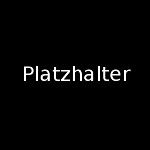
\includegraphics[scale=1.0]{spacer}
		\caption{Das KinPro System}
		\label{fig.kinpro}
	\end{center}
	%\vspace*{-8mm}
\end{figure}

\subsection{Kamerakalibrierung}
Die Kalibrierung der RGB-Kamera erfolgt 

\subsection{Begriffe und Notationen}
Es sollen zunächst einige Begriffe und Notationen definiert werden, um eine konsistente Beschreibung im Verlaufe dieser Arbeit zu ermöglichen.\\
In Anlehnung an die Literatur \cite{Zhang2000} werden 2D-Punkte mit \pteq{x,y} und 3D-Punkte mit \pteq[P]{X,Y,Z} bezeichnet. Die gleiche Darstellung wird auch für Vektoren und Matrizen verwendet, wobei die Ausnahme der für die Punktbeschreibung verwendete Buchstabe P bildet. Es werden demnach Vektoren über \vec{v} und Matrizen mit \vec{M} beschrieben.\\
Mittels der homogenen Koordinatendarstellung lassen sich Punkte gleichzeitig sowohl translatorisch als auch rotatorisch transformieren. Dazu wird der \textit{inverse Streckungsfaktor} als zusätzliche Komponente eingeführt, für welchen standardmäßig $w=1$ gilt \cite{Nischwitz20111}. Zur Unterscheidung werden homogene Koordinaten damit zu \ptheq{x,y} bzw. \ptheq[P]{X,Y,Z} definiert.\\
Falls nicht mittels eines vorangestellten Index $\ve{i}{p}$ anders gekennzeichnet bezieht sich die Darstellung von Punkten und Körpern immer auf das globale Koordinatensystem, welches mit $\ks{0}$ bezeichnet wird. Transformationsvorschriften zwischen zwei Koordinatensystemen $\ks{j}$ und $\ks{k}$ werden mit Hilfe der Matrixschreibweise als $\tmat{j}{k}$ ausgedrückt.\\
Die Transformation, die einen Punkt vom Koordinatensystem des Projektors ($\ks{P}$) in das globale Koordinatensystem abbildet, lässt sich beispielsweise demnach als
\begin{equation}
\ve{0}{p} = \tmat{0}{P}\ve{P}{p}
\end{equation}
ausdrücken.\\
Weiterhin werden die in der Literatur verbreiteten Konventionen für die Darstellung und Orientierung von Koordinatensystemen verwendet: Die farbliche Zuordnung der Koordinatenachsen richtet sich nach der RGB Darstellung. Die X-Achsen werden somit rot, die Y-Achsen grün und die z-Achsen blau eingefärbt abgebildet. Bei Kameras und Projektoren wird die Orientierung der körpereigenen Koordinatensysteme darüber hinaus so gewählt, dass die Z-Achse in Richtung der optischen Achse ausgerichtet wird.\\ \abb{fig.coords}
\begin{figure}[ht]
	\begin{center}
		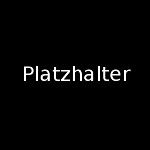
\includegraphics[scale=1.0]{spacer}
		\caption{Darstellung von Koordinatensystemen am Beispiel der Kinect}
		\label{fig.coords}
	\end{center}
	%\vspace*{-8mm}
\end{figure}

\subsection{Lochkameramodell / Kameragrundlagen}
Das einfachste Modell einer Kamera bildet das sogenannte Lochkameramodell. Dabei wird von einer Kamera ohne Optik ausgegangen, welche eine infinitesimal kleine Blendenöffnung besitzt. Die Abbildung eines dreidimensionalen Objektes in die Bild bzw. Sensorebene der Kamera kann damit über das optische Zentrum $C$ im Ursprung des Kamerakoordinatensystems $\ks{K}$ und die Brennweite $f$ beschrieben werden. Die Brennweite charakterisiert dabei den Abstand zwischen der Brenn- und der Bildebene. Um die gespiegelte Abbildung in der Bildebene der Darstellung des Modells zu vermeiden wird in den folgenden Erläuterungen eine Punktspiegelung der Brennebene vorausgesetzt, so dass diese vor das optische Zentrum gelegt wird. Das beschriebene Modell der Lochkamera ist in \abb{fig.pinhole} dargestellt.\\
\red[\cite{Suesse2014} \cite{Roehl}]
\red[Kamerakoordinatensystem als C statt K!?]

\begin{figure}[ht]
	\begin{center}
		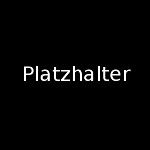
\includegraphics[scale=1.0]{spacer}
		\caption{Modell der Lochkamera mit den Ebenen}
		\label{fig.pinhole}
	\end{center}
	%\vspace*{-8mm}
\end{figure}

Anhand des $\tan{\alpha}$\red[alpha?] des jeweiligen in die Ebene projizierten Strahlenwinkels lassen sich leicht die Beziehungen zwischen den Koordinaten eines Objektpunktes $\ve{K}{P} = [X_K, Y_K, Z_K]$ und seiner Abbildung in der Brennebene $\ve{B}{p} = [x_B, y_B]$ herleiten:
\begin{equation}
\frac{x_B}{f}=\frac{X_K}{Z_K} \quad \rightarrow \quad x_B = \frac{f\cdot X_K}{Z_K}
\label{eq.xf}
\end{equation}
\begin{equation}
\frac{y_B}{f}=\frac{Y_K}{Z_K} \quad \rightarrow \quad y_B = \frac{f\cdot Y_K}{Z_K}
\label{eq.yf}
\end{equation}

Durch Umformung von \eq{eq.xf} und \eq{eq.yf} und unter Verwendung der homogenen Koordinaten lässt sich die Abbildungsgleichung damit darstellen als:
%\begin{equation}
%Z_K\cdot
%\left(\begin{array}{c}
%x_B\\
%y_B\\
%1\\
%\end{array}\right) = \left(\begin{array}{cccc}
%f & 0 & 0 & 0\\
%0 & f & 0 & 0\\
%0 & 0 & 1 & 0\\
%\end{array}\right)\cdot\left(\begin{array}{c}
%X_K\\
%Y_K\\
%Z_K\\
%1\\
%\end{array}\right)  
%\label{eq.perspProj}
%\end{equation}
\begin{equation}
\left(\begin{array}{c}
x_B\\
y_B\\
1\\
\end{array}\right) = \left(\begin{array}{cccc}
\frac{f}{Z_K} & 0 & 0 & 0\\
0 & \frac{f}{Z_K} & 0 & 0\\
0 & 0 & \frac{1}{Z_K} & 0\\
\end{array}\right)\cdot\left(\begin{array}{c}
X_K\\
Y_K\\
Z_K\\
1\\
\end{array}\right)  
\label{eq.perspProj}
\end{equation}

Wie aus \eq{eq.persProj} hervorgeht ist damit die perspektivische Projektion des Punktes in die Bildebene bis auf den Faktor $Z_K$ eindeutig beschrieben. Es wird daher der Skalierungsfaktor $s=Z_K$ eingeführt, so dass sich \eq{eq.persProj} mit der perspektivischen Projektionsmatrix $\tmat{B}{K}$ zusammenfassen lässt zu:
\begin{equation}
s\cdot\ve{B}{\tilde{p}} = \tmat{B}{K}\ve{K}{\tilde{P}}
\end{equation}

\red[
Notation\\
Lochkameramodell\\
Intrinsische + Extrinsische Parameter\\
Kalibrierung Kamera (RGB+IR)\\
Tiefeninformationen (Epipolargeometrie etc.)\\
Projektor als inverse Kamera\\
Kalibrierung Projektor + Kamera+Projektor\\
Transformationen zwischen den Koordinatensystemen (oder in Kapiteln erst?)
]

Wichtig sind die Transformationen zwischen den Koordinatensystemen und die Abbildung des Projektors. Die Transformation erfolgt allerdings immer über die Kamera, da diese im Weltkoordinatensystem lokalisiert wird. Für die Kalibrierung sind die intrinsischen und extrinsischen Parameter relevant, aber auch die Herkunft?

\section{Software}
Zur Realisierung der einzelnen Systemfunktionen wurden Komponenten erstellt, welche auf verschiedenen Softwarebibliotheken aufgebaut sind. Die Bedienfunktionen des Systems wurden dabei innerhalb einer grafischen Benutzeroberfläche zusammengefasst. Bevor die Programmstruktur näher erläutert wird sollen deshalb zunächst die verwendeten Bibliotheken und Softwareumgebungen dargestellt werden.

\subsection{ROS}
\label{chap:ros}
Das Robot Operating System (ROS) ist eine speziell für die Anwendung in der Robotik entwickelte, quell-offene Sammlung aus Softwarebibliotheken \cite{ROS}. Neben Treibern für verschiedene Hardwarekomponenten und speziellen Algorithmen bietet ROS eine Umgebung welche die Integration von und Kommunikation zwischen verschiedenen Modulen vereinfacht um komplexe und robuste Anwendungen zu realisieren. \red[Hertzberg Buch detaillierter]

\subsection{Open Source Computer Vision Library}
Die Open Source Computer Vision Library (OpenCV) ist eine quell-offene Bibliothek aus Funktionen und Algorithmen zur Anwendung in der Bild- und Videoverarbeitung \cite{OpenCV}. Nachdem OpenCV ursprünglich von einer Forschungsgruppe bei Intel entwickelt wurde \cite{Laganiere2011}, wird die Bibliothek heute von einer großen Anzahl an Firmen und Entwicklern verwendet und ständig weiterentwickelt. Sie umfasst mittlerweile mehr als 2500 optimierte Algorithmen zur Anwendung in Bereichen wie Objekterkennung, Segmentierung oder Navigation.

\subsection{Point Cloud Library}
Punktwolken sind Datenstrukturen, welche eine Sammlung multidimensionaler Punkte repräsentieren. Diese Struktur wird verwendet um die von der Kinect aufgenommenen Tiefeninformationen darzustellen und weiter verarbeiten zu können. Die Point Cloud Library (PCL) wurde mit dem Ziel entwickelt, ein Rahmenwerk zu schaffen, welches die Verarbeitung von Punktwolken mittels verschiedener Algorithmen ermöglicht. Ähnlich wie OpenCV für die 2D Bildverarbeitung wird PCL bezogen auf Punktwolken in den Bereichen Objekterkennung, Segmentierung oder Filterung angewendet. Auch PCL ist eine quell-offene Bibliothek, welche von einer Vielzahl an Firmen und Entwicklern ständig überarbeitet und erweitert wird \cite{PCL}.

\subsection{Qt}
Die von der Firma Trolltech entwickelte und mittlerweile von der Firma Digia verwaltete Qt Bibliothek ermöglicht eine plattformunabhängige Entwicklung von grafischen Benutzerschnittstellen im C++ Standard \cite{Qt}. Die Qt Bibliothek wurde in dieser Arbeit verwendet um die Schnittstelle zu realisieren mit welcher der Benutzer Zugriff auf die Funktionen der verschiedenen Programmkomponenten erhält.

\subsection{Visualization Toolkit}
Das Visualization Toolkit (VTK) stellt eine auf dem C++ Standard basierende Bibliothek dar, welche für die Verarbeitung und Visualisierung von 3D Bilddaten entwickelt wurde. Die Firma Kitware entwickelt die Bibliothek ständig weiter und stellt sie als quell-offene Software zur Verfügung \cite{VTK}. Verschiedene Schnittstellen zwischen VTK und PCL ermöglichen neben der Darstellung von 3D Objekten auch die Integration und Visualisierung von Punktwolken.

\subsection{GUI/Programmstruktur}
\red[Mit aufnehmen in dieser Liste?]
Die für die Anwendung des Kamera-Projektor-Systems als selbstlokalisierendes, handgeführtes Projektionssystem entwickelte Software umfasst verschiedene Module, welche durch ROS verknüpft werden. Dies ermöglicht den Informationsaustausch zwischen den Komponenten auf Basis definierter Daten- und Kommunikationsstrukturen. Der Austausch einzelner Komponenten ist damit jederzeit möglich, sodass die Entwicklung und Integration optimierter Module je nach Anwendungsgebiet vorgenommen werden kann.\\
Einen Überblick über die einzelnen Funktionsmodule, ihre Verknüpfung untereinander und die Schnittstelle zum Benutzer zeigt Abbildung \ref{fig.modules}.\\

Module: \mLocalization - EKF Odometrie (Tracking) - Visuelle Odometrie - IMU - Visualisierung - Transformation - Interaktion - Benutzeroberfläche - Projektion - Kartenserver

\begin{figure}[ht]
	\begin{center}
		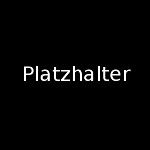
\includegraphics[scale=1.0]{spacer}
		\caption{Funktionsmodule der Anwendungssoftware}
		\label{fig.modules}
	\end{center}
	%\vspace*{-8mm}
\end{figure}

Das \mLocalization bestimmt und überwacht die aktuelle Position des Kamera-Projektor-Systems. Es ermittelt die initiale Position mittels globaler Lokalisation auf Basis der vom \mMapserver zur Verfügung gestellten Karte. Als weitere Eingangsgröße verwendet es die Odometriedaten, welche vom \mEkf zur Verfügung gestellt werden um Veränderungen in der Position während der Bedienung zu erkennen und die Positionsdaten dementsprechend zu aktualisieren. Das \mEkf selbst verwendet und filtert dabei die visuellen Odometriedaten des \mFovis und die Lagedaten des \mImu \red[TODO Moduls] um die kombinierten Odometriedaten zu bestimmen.\\
Diese so vom \mLocalization bestimmten Positionsdaten werden dann dem \mTransformation übermittelt, welches alle Koordinatentransformationen zwischen der ermittelten Kameraposition, dem Projektor und den relevanten Objekten der Umgebung berechnet. Diese Berechnungen werden dann vom \mVisualization verwendet, um ein Abbild der aktuellen Projektorsicht innerhalb der 3D Umgebung zu erstellen. Diese Ansicht wird dem Benutzer anschließend sowohl über die Benutzeroberfläche durch das \mGui als auch über die Projektion durch das \mProjection dargestellt. Das \mInteraction erkennt vom Benutzer durchgeführte Gesten oder Bewegungen, über welche er auf Basis der projizierten Daten mit der Modellumgebung interagiert. Die Steuerungsbefehle werden dann über das \mTransformation an das \mVisualization übertragen, wo diese interpretiert werden und in Form von Modifikationen der Modellumgebung umgesetzt werden.\\
Die jeweilige spezifische Realisierung der Module wird in den folgenden Kapiteln näher spezifiziert.
